\documentclass[../main.tex]{subfiles}

\begin{document}

\begin{boxnaslovi}
\section{Logičko programiranje}
\end{boxnaslovi}

Imperativnu paradigmu karakteriše postojanje naredbi, sekvenci, selekcija, iteracija i propratnih efekata. Funkciopnalnu paradigmu karakteriše evaluacija funkcija korišćenjem redukcija. U logičkoj paradigmi imamo logičke metode (na primer metod rezolucije).
\\
Pomenute paradigme se temelje na različitim teorijskim modelima:
\begin{description}

\item[Formalizam za imperativne jezike -- Tjuringova mašina] \hfill

	Imperativni jezici imaju svu izražajnost Tjuringove mašine (uz ograničenje memorije i resursa).

\item[Formalizam za funkcionalne jezike -- Lambda račun] \hfill

	Funkcionalni jezici imaju svu izražajnost lambda računa (uz ograničenje memorije i resursa).
	
\item[Formalizam za logičke jezike -- Logika prvog reda] \hfill

	Logika prvog reda {\it nije} formalizam izračunljivosti, tako da je teško vršiti poređenje ove vrste. Ipak, većina logičkih jezika je Tjuring-kompletno.
\end{description}

\subsection{Rešavanje problema}

U logičkom programiranju, logika se koristi kao deklarativni jezik za opisivanje problema, a dokazivač teorema kao mehanizam za rešavanje problema. Rešavanje problema je podeljeno između programera koji opisuje problem i dokazivača teorema koji problem rešava.
\\
Sintaksa opisa problema je dosta slična u jezicima logičke paradigme, ali dokazivač teorema može da se razlikuje. Najznačajniji predstavnik logičke paradigme je Prolog, koji se često koristi i kao sinonim za logičku paradigmu.
\\
U procesu rešavanja problema, Prolog koristi metod rezolucije.

\subsection{Razvoj logičkog programiranja}
{\renewcommand{\arraystretch}{1.2}
\begin{tabularx}{\textwidth}{>{\hsize=.2\hsize}r|X}
1879. & G.Frege -- Predikatski račun (sredstvo za analizu formalne strukture čistog mišeljenja) \\
1915-1936.& Gedel, Erban, Skulem, Turing,... Osnovi teorije izračunljivosti \\
1965.& J.A.Robinson, Metod rezolucije \\
\hline
1967. & Prvi logički jezik - ABSYS - Aberdeen SYStem M.Foster, T.Elkok, Group for Computing Research, University of Aberdeen (UK) Radi sa tvrđenjima (aksiomama) preko kojih se, nakon postavljanja pitanja, deduktivnim putem generiše odgovor. ABSYS je antipicira razne koncepte koji se kasnije koriste u logičkom programiranju.\\
\hline
{\bf Razvoj Prologa} & \\
\hline
1971. &Pod rukovodstvom A.Colmerauer-a u Marselju kreiran Q-System (obrada prirodnih jezika). \\
1972. &Q-System preimenovan u PROLOG (PROgramming in LOGic). Saradnja sa Robertom Kovalskim iz Edinburga (automatsko dokazivanje). Implementiran prvi interpretator za Prolog. (Saradnici: Ph. Roussel, R.Pasero, J.Trudel) \\
1974. &Na kongresu IFIP-a (International Federation for Information Processing)  R.Kavalski predstavio Prolog široj javnosti. \\
1977. &David Warren napravio efikasnu implementaciju kompajlera za Prolog za DEC-10
u Edinburgu. (Edinburški Prolog). Osnova sintakse za moderan Prolog. \\
1981. &Seminari u Sirakuzi i Los Anđelesu. \\
1982. &Prva međunarodna konferencija o Prologu u Marselju.\\
1983. &Japanski projekat o razvoju računara 5. generacije. \\
1986. &The Association for Logic Programming http://www.logicprogramming.org/ \\
1993.& Završen Japanski projekat razvoja računara 5. generacije.\\
1995.& ISO Prolog standard \\
2007,2012. & Korekcije standarda, dodavanje modula.
\end{tabularx}
}
\\ \\
Prolog se često koristi kao sinonim za logičko programiranje. Nakon početnih godina intenzivnog razvoja jezika, sada je razvoj usmeren ka integracijama jezika sa drugim programskim jezicima. I dalje se istražuju efikasniji algoritmi za prevođenje Prolog programa u izvršni kod. Razne implementacije Prologa: BProlog, GNU Prolog, JIProlog, Visual Prolog, SWI Prolog,...
Prolog je uticao na razvoj raznih programskih jezika: ALF, Fril, Godel, Mercury, Oz, Ciao, Visual Prolog, XSB, $\lambda$Prolog,...

\subsection{Drugi predstavnici logičke paradigme}
Pored Prologa, značajni predstavnici logičke paradigme su i {\bf ASP} (Answer Set Programming) i {\bf Datalog}. Sintaksa Dataloga i jezika koji pripadaju ASP podparadigmi su veoma slične Prologu, ali se proces rešavanja problema razlikuje.
ASP za izračunavanje ne koristi metod rezolucije već rešavače za iskaznu logiku. Koristi se najčešće za pretragu kod NP teških problema, npr bojenje grafova, hamiltonovi ciklusi, velike klike,...
\\
Datalog (logic and databases) je u sintaksnom smislu podskup Prologa koji se koristi za integraciju podataka, izvlačenje podataka, umrežavanje, analizu programa, cloud computing. Datalog može da koristi različite efikasne algoritme za odreživanje vrednosti upita. Datalog  nije Tjuring kompletan.


\subsection{Primena}
\begin{multicols}{2}
Logičko programiranje je {\it pogodno} za:
\begin{itemize}
	\item rešavanje problema matematičke logike
	\item obradu prirodnih jezika
	\item podršku relacionim bazama podataka
	\item automatizaciju projektovanja
	\item simboličko rešavanje jednačina
	\item razne oblasti veštačke inteligencije
\end{itemize}
\end{multicols}
{\it Nije pogodno} za: 
	I/O algoritme, 
	grafiku, 
	numeričke algoritme.

\subsection{Logika prvog reda - osnovni pojmovi}
\subsubsection{Sintaksa}
\begin{description}
\item[Logički deo jezika prvog reda čine:] \hfill

\begin{itemize}
	\item skup promenljivih $V$
	\item skup logičkih veznika $\{ \neg, \wedge, \vee, \Rightarrow, \Leftrightarrow \}$
	\item skup kvantifikatora $\{ \exists, \forall \}$
	\item skup logičkih konstanti $\{ \top, \bot \}$
	\item skup pomoćnih simbola $\{ (,  ) \}$
\end{itemize}
Elementi ovih skupova nazivaju se logički simboli.

\item[Rečnik ili signatura] \hfill

{\bf Rečnik} ili signatura sastoje se od najviše prebrojivih skupova $\sum$ i $\prod$ koje redom nazivamo skupom {\bf funkcijskih simbola} i skupom {\bf predikatskih simbola}, kao i od funckije $ar$ koja preslikava uniju ovih skupova u nenegativne cele brojeve i koju nazivamo {\bf arnost}.
\\
Presek svaka dva od prethodno nabrojanih skupova je prazan. Funkcijske simbole arnosti 0 zovemo simbolima konstanti. Skupovi $\sum$ i $\prod$ čine nelogički deo jezika prvog reda, a sve njihove elemente zovemo {\bf nelogičkim simbolima}.

\item[Term] \hfill

Skup {\bf termova} nad signaturom $\mathcal{L} = (\sum, \prod, ar)$ i skupom promenljivih $V$ je skup za koji važi:
\begin{itemize}
	\item svaki simbol konstante (tj. svaki funkcijski simbol arnosti 0) je term
	\item svaki simbol promenljive je term
	\item ako je $f$ funkcijski simbol za koji je $ar(f) = n$ i $t_1,t_2, \ldots, t_n$ su termovi, onda je i $f(t_1, t_2, \ldots, t_n)$ term
\end{itemize}
Termovi se mogu dobiti samo konačnom primenom prethodnih pravila.

\item[Atomičke formule] \hfill

Skup {\bf atomičkih formula} nad signaturom $\mathcal{L} = (\sum, \prod, ar)$ i skupom promenljivih $V$ je skup za koji važi:
\begin{itemize}
	\item logičke konstante $\top$ i $\bot$ su atomičke formule 
	\item ako je $p$ predikatski simbol za koji je $ar(p)=n$ i $t_1,t_2, \ldots, t_n$ su termovi, onda je $p(t_1, t_2, \ldots, t_n$ atomička formula.
\end{itemize}

\item[Dobro zasnovane formule (ili samo formule)] \hfill

Skup {\bf dobro zasnovanih formula} nad signaturom $\mathcal{L} = (\sum, \prod, ar)$ i skupom promenljivih $V$ je skup za koji važi:
\begin{itemize}
	\item svaka atomička formula je dobro zasnovana formula
	\item ako je $A$ dobro zasnovana formula, onda je i $(\neg A)$ dobro zasnovana formula
	\item ako su $A$ i $B$ dobro zasnovane formule, onda su i $(A\wedge B)$, $(A\vee B)$, $(A\Rightarrow B)$ i $(A \Leftrightarrow B)$ dobro zasnovane fomule 	
	\item ako je $A$ dobro zasnovana formula i $x$ je promenljiva, onda su i $((\forall x)A)$ i $((\exists x)A)$ dobro zasnovane formule.
\end{itemize}
	Dobro zasnovane formule se mogu dobiti samo konačnom primenom prethodnih pravila.

\item[Osnovni pojmovi] \hfill

{\bf Literal} je atomička formula ili negacija atomičke formule.\\
{\bf Klauza} je disjunkcija literala. \\
Pod terminom {\bf izraz} podrazumevaju se termovi i (dobro zasnovane) formule. 
\end{description}

\subsubsection{Supstitucija i unifikacija}
\begin{description}

\item[Supstitucija za term] \hfill

Term dobijen zamenom (supstitucijom) promenljive $x$ termom $t_x$ u termu $t$ označavamo sa  $t[x\mapsto t_x]$ i definišemo na sledeći način:
\begin{itemize}
\item ako je $t$ simbol konstante, onda je $t[x\mapsto t_x]=t$
\item ako je $t=x$, onda je $t[x\mapsto t_x]=t_x$
\item ako je $t=y$, gde je $y\neq x$, onda je $t[x\mapsto t_x]=t$
\item ako je $t=f(t_1, t_2, \ldots, t_n)$, onda je $t[x\mapsto t_x]=f(t_1[x\mapsto t_x], t_2[x\mapsto t_x], \ldots, t_n[x\mapsto t_x])$
\end{itemize}

\item[Supstitucija za formule] \hfill

Formulu dobijenu zamenom (supstitucijom) promenljive $x$ termom $t_x$ u formuli $\mathcal{A}$ označavamo sa $\mathcal{A}[x\mapsto t_x]$ i definišemo na sledeći način:
\begin{itemize}
\item $\top[x\mapsto t_x]=\top$

\item $\bot[x\mapsto t_x]=\bot$

\item ako je $\mathcal{A}=p(t_1, t_2, \ldots, t_n)$, onda je $\mathcal{A}[x\mapsto t_x]=p(t_1[x\mapsto t_x], t_2[x\mapsto t_x], \ldots, t_n[x\mapsto t_x])$

\item $(\neg \mathcal{A})[x\mapsto t_x]=\neg(\mathcal{A}[x\mapsto t_x])$

\item $(\mathcal{A}\vee \mathcal{B}  )[x\mapsto t_x]=(\mathcal{A}[x\mapsto t_x] \vee  \mathcal{B}[x\mapsto t_x] )$

\item $(\mathcal{A} \wedge \mathcal{B})[x\mapsto t_x]=(\mathcal{A}  [x\mapsto t_x] \wedge  \mathcal{B}[x\mapsto t_x] )$

\item $(\mathcal{A} \Rightarrow  \mathcal{B})[x\mapsto t_x]=(\mathcal{A}  [x\mapsto t_x] \Rightarrow \mathcal{B}[x\mapsto t_x] )$

\item $(\mathcal{A} \Leftrightarrow \mathcal{B})[x\mapsto t_x]=(\mathcal{A}  [x\mapsto t_x] \Leftrightarrow \mathcal{B}[x\mapsto t_x] )$

\item $(\forall x\mathcal{A})[x\mapsto t_x] = (\forall x\mathcal{A})$

\item $(\exists x\mathcal{A})[x\mapsto t_x] = (\exists x\mathcal{A})$

\item ako je $x\neq y$, neka je $z$ promenljiva koja se ne pojavljuje ni u $(\forall y)\mathcal{A}$ ni u $t_x$;  \hfill

tada je $(\forall y\mathcal{A})[x\mapsto t_x] = (\forall z)\mathcal{A}[y\mapsto z][x\mapsto t_x]$

\item ako je $x\neq y$, neka je $z$ promenljiva koja se ne pojavljuje ni u $(\exists y)\mathcal{A}$ ni u $t_x$; \hfill
 
 tada je $(\exists y\mathcal{A})[x\mapsto t_x] = (\exists z)\mathcal{A}[y\mapsto z][x\mapsto t_x]$
\end{itemize}
Primetimo da poslednja dva pravila u prethodnoj definiciji obezbeđuju, na primer, da 
$((\forall y)p(x,y))[x\mapsto y]$ ne bude $(\forall y)p(y,y)$ već $(\forall z)p(y,z)$.

\item[Uopštena zamena (supstitucija)] \hfill

Uopštena zamena (supstitucija) $\sigma$ je skup zamena $[x_1\mapsto t_1], [x_2\mapsto t_2], \ldots, [x_n\mapsto t_n]$ gde su $x_i$ promenljive i $t_i$ su proizvoljni termovi i gde je $x_i\neq x_j$ za $i\neq j$. Takvu zamenu zapisujemo kraće $[x_1\mapsto t_1, x_2\mapsto t_2, \ldots, x_n\mapsto t_n]$
\\
Uopštena zamena primenjuje se simultano na sva pojavljivanja promenljivih $x_1, x_2, \ldots, x_n$ u polaznom izrazu i samo na njih (tj. ne primenjuje se na podtermove dobijene zamenama). Izraz koji je rezultat primene zamene $\sigma$ nad izrazom $E$, označavamo sa $E\sigma$.

\begin{boxprimer}
\begin{itemize}
\item Za $\sigma = [x\mapsto f(y)]$ i $s=g(a,x)$ važi $s\sigma=g(a,f(y))$
\item Za $\sigma = [x\mapsto f(x)]$ i $s=g(a,x)$ važi  $s\sigma=g(a,f(x))$
\item Za $\sigma = [x\mapsto f(y), y\mapsto a], s=g(a,x)$ i $t=g(y,g(x,y))$ važi  $s\sigma=g(a,f(y))$ i $t\sigma=g(a, g(f(y),a) )$
\end{itemize}
\end{boxprimer}

\item[Unifikacija] \hfill

Problem unifikacije je problem ispitivanja da li postoji supstitucija koja čini dva izraza (dva terma ili dve formule) jednakim.\\
Ako su $e_1$ i $e_2$ izrazi i ako postoji supstituija $\sigma$ takva da važi $e_1 \sigma=e_2 \sigma$ onda kažemo da su izrazi $e_1$ i $e_2$ {\bf unifikabilni} i da je supstitucija $\sigma$ {\bf unifikator} za ta dva izraza. Dva unifikabilna izraza mogu da imaju više unifikatora.

\begin{boxprimer}
Primeri unifikacije: \\
\begin{tikzpicture}[node distance = 1cm]
\node at (0.5 , 1) (top1)  {$d$};
\node at (0 , 0)   (n1)  {$a$} 
 	edge[](top1.south);
\node at (1 , 0)  (n2) {$X$} 
	edge[](top1.south);

\node at ( 2.5, 1 ) (top2) {$d$};
\node at ( 2 , 0 ) (n3) {$a$}
	edge(top2.south);
\node at ( 3 , 0 ) (n4) {$b$}
	edge(top2.south);

\node at (4, 0.5) {$\{X=b\}$};

\node at (0.5, -1) (top3) {$s$};
\node at (0, -2.5) (n5) {$Y$}
	edge(top3.south);
\node at (1, -2.5) (n7) {$X$}
	edge(top3.south);
\node at (0.5,-2.5) (n6) {$a$};
\coordinate (n7') at ($(top3)!0.5!(n7)$);
\draw (n7') -- (n6);
	
\node at (2.5, -1) (top4) {$s$};
\node at (2, -2.5) (n8) {$X$}
	edge(top4.south);
\node at (3, -2.5) (n10) {$b$}
	edge(top4.south);
\node at (2.5,-2.5) (n9) {$Y$};
\coordinate (n10') at ($(top4)!0.5!(n10)$);
\draw (n10') -- (n9);

\node at (5, -2) {Nemoguća unifikacija};


\node at (8, 0) (top5) {};
\node at (7.5, -1) (n11) {$X$}
	edge(top5.south);
\node at (8.5, -1) (n13) {$X$}
	edge(top5.south);
\node at (8, -1) (n12) {$a$};
\coordinate (n13') at ($(top5)!0.5!(n13)$);
\draw (n13') -- (n12);

\node at (10,0) (top6) {};
\node at (9.5, -1) (n14) {$b$}
	edge(top6.south);
\node at (10.5, -1) (n16) {$Z$}
	edge(top6.south);
\node at (10, -1) (n15) {$Y$};
\coordinate (n16') at ($(top6)!0.5!(n16)$);
\draw (n16') -- (n15);

\node at (13,-0.5) {$\{X=b, Y=a, Z=b\}$};

\end{tikzpicture}

\end{boxprimer}

Neka je term $t_1$ jednak $g(x,z)$, neka je term $t_2$ jednak $g(y,f(y))$ i neka je $\sigma$ supstitucija $[y \mapsto x, z\mapsto f(x)]$. Tada je i $t_1\sigma$ i $t_2\sigma$ jednako $g(x,f(x))$, pa su termovi $t_1$ i $t_2$ unifikabilni, a $\sigma$ je (jedan) njihov unifikator.
\begin{boxprimer}[width=\linewidth/3*2]
Unifikator termova $t_1$ i $t_2$ je npr. i $[x\mapsto a, y\mapsto a, z\mapsto f(a)]$
\\
Termovi $g(x,x)$ i $g(y,f(y))$ nisu unifikabilni.
\end{boxprimer}
Među svim unifikatorima za dva izraza postoji jedan koji je najopštiji, tj. svi drugi se mogu dobiti iz njega primenom dodatne supstitucije. 

\begin{boxprimer}
Ako imamo termove $f(x)$ i $f(y)$ i supstitucije $\sigma_1 = [x\mapsto a, y\mapsto a]$ , $\sigma_2 = [x\mapsto b, y\mapsto b]$ i $\sigma = [x\mapsto y]$ u ovom slučaju $\sigma$ je najopštiji unifikator.
\end{boxprimer}

Postoji algoritam koji pronalazi {\bf najopštiji unifikator} i vraća neuspeh ukoliko identifikator za dva izraza ne postoji.

\end{description}

\subsubsection{Metod rezolucije}
Metod rezolucije je metod za izvođenje zaključaka (logičkih posledica) u logici prvog reda koji se zasniva na pravilu rezolucije. Na primer, posledica formula $A \Rightarrow B$ i $B\Rightarrow C$ je formula $A \Rightarrow C$. Navedeni zaključak ne bi mogao da se izvede iz formula $A \Rightarrow B'$ i $B'' \Rightarrow C$. Međutim, ukoliko su $B'$ i $B''$ unifikabilni, onda se oni mogu učiniti jednakim za neko $\sigma$ pa je posledica formula $A\sigma \Rightarrow B'\sigma$ i $B''\sigma \Rightarrow C\sigma$ upravo $A\sigma \Rightarrow C\sigma$. Zapravo, pravilo rezolucije se iskazuje u terminima klauza, tj. $\neg A \vee B$ i $\neg B \vee C$ daje $\neg A \vee C$.


\begin{boxnaslovi}
\section{Prolog}
\end{boxnaslovi}

\subsection{Teorijske osnove}
Kao što se Haskell oslanja na lambda račun, tako se Prolog oslanja na logiku prvog reda i metod rezolucije. Potrebno je poznavanje pojmova iskazne logike i logike prvog reda. Prološki zapis programa je izveden iz zapisa formula logike prvog reda. Ovaj zapis je redukovani zapis formula logike prvog reda -- ne mogu se sve formule logike prvog reda izraziti u Prologu. U Prologu se mogu izraziti samo {\bf Hornove klauze}. Hornova klauza je {\it disjunkcija literala sa najviše jednim nenegiranim literalom}.
\begin{multicols}{2}
Hornova klauza odgovara implikaciji
\begin{center}
$(A_1 \wedge A_2 \wedge \ldots \wedge A_n) \Rightarrow B$\\
$\Longleftrightarrow$\\
$\neg(A_1 \wedge A_2 \wedge \ldots \wedge A_n) \vee B$\\
$\Longleftrightarrow$\\
$\neg A_1 \vee\neg A_2 \vee \ldots \vee\neg A_n \vee B$\\
\end{center}

\columnbreak
\noindent Hornove klauze u Prologu se zapisuju u obliku:
$$ B\Leftarrow (A_1 \wedge A_2 \wedge \ldots \wedge A_n)  $$
pri čemu se znak $\Leftarrow$ zapisuje kao \texttt{:-}
\\ \texttt{B:-(A1, A2,\ldots, An)}
\end{multicols}

Hornove klauze omogućavaju efikasnu primenu metoda rezolucije. One predstavljaju ograničenje: ne može se izraziti tvrđenje oblika $\neg A\Rightarrow B$. Prethodnom tvrđenju odgovara formula $A\vee B$, dakle formula koja sadrži dva nenegativna literala.
\\
Supstitucija je preslikavanje koje promenljive preslikava u termove. Supstitucija se sastoji od konačnog broja pravila preslikavanja, npr. $x\rightarrow a, y\rightarrow f(a,b), u\rightarrow v$.
\\
Dva terma $t$ i $u$ se mogu unifikovati ako i samo ako postoji supstitucija $\sigma$ tako da vazi $t\sigma = u\sigma$. Unifikacija se koristi prilikom traženja rešenja u okviru Prologa.

\begin{multicols}{2}
Programiranje u Prologu se sastoji u
\begin{itemize}
\item obezbeđivanju činjenica o objektima i odnosima među njima 
\item definisanju pravila o objektima i odnosima među njima
\item formiranju upita o objektima i odnosima među njima
\end{itemize}
\columnbreak
\begin{boxprimer}
\begin{Verbatim}
?- write(`Hello world!'), nl.
Hello world!
true.
\end{Verbatim}
\end{boxprimer}
\end{multicols}

\subsection{Sintaksa}
{\bf Termovi} su {\it osnovni gradivni elementi }Prologa i širi su od pojma terma logike prvog reda, tj.  \textcolor{red}{ $$Term\_Prologa \neq Term\_logike\_prvog\_reda $$}.

\begin{figure}[h!]

\begin{tikzpicture}[sibling distance=10em, 
  every node/.style = {shape=rectangle, rounded corners, draw, align=center}, yellowNode/.style={fill=yellow}, redoranNode/.style={fill = redorange}, 
  thistNode/.style={fill=thistle}]
\tikzstyle{level 2}=[sibling distance=5cm]
\tikzstyle{level 3}=[sibling distance=2cm]
  
\node[fill=seagreen] {Term}
	child { node[yellowNode] {Konstanta}
		child { node[redoranNode] {Atom}
			child{ node[thistNode] {AlfaNum.}  
			}
			child{ node[thistNode] {SpecZn.}  
			}
			child{ node[thistNode] {Apostrofni}  
			}
		}
		child { node[redoranNode] {Broj}
			child{ node[thistNode] {Ceo}  
			}
			child{ node[thistNode] {Realni}  
			}
		}		
	 }
	child { node[yellowNode] {Promenljiva} }
	child { node[yellowNode] {Struktura} };
 
\end{tikzpicture}
\caption{Sintaksa}
\label{fig:sintaksa}
\end{figure}

Promenljive se zapisuju velikim početnim slovom ili simbolom \texttt{\_} (simboim \texttt{\_} počinju {\it imena anonimnih promenljivih čije vrednosti nisu bitne}). Strukture ili predikati se grade od atoma i termova. Ako je $p$ atom, a $t_1, t_2, \ldots, t_n$ termovi, onda je $p(t_1, t_2, \ldots, t_n)$ term.

\subsection{Programi}

\begin{multicols}{2}
\indent {\bf Činjenice} su Hornove klauze bez negiranih literala (dakle, samo B).  Pomoću činjenica opisuju se svojstva \break objekata, odnosno relacije između objekata.

\begin{boxprimer}
\begin{verbatim}
zivotinja(panda) .
biljka(bambus) .
jede(panda, bambus) .
\end{verbatim}
\end{boxprimer}

\end{multicols}
Činjenice su konstrukcije Prologa koje se sastoje iz {\bf funktora} iza kojih slede argumenti između malih zagrada. 
Ukoliko ima više argumenata, razdvajaju se zapetama. Funktor predstavlja {\it naziv relacije}, a argumenti nazive objekata.
Imena činjenica treba zadavati u skladu sa njihovim značenjem(semantikom). Prolog prihvata činjenice kao {\it apsolutne istine} (aksiome) i ne proverava njihovu tačnost.
\begin{multicols}{2}
\begin{boxprimer}
U tom smislu činjenice u Prologu su:
\begin{verbatim}
biljka(panda) .
zivotinja(bambus) .
jede(bambus, panda) .
\end{verbatim}
\end{boxprimer}
Skup činjenica formira {\it bazu činjenica} (bazu podataka).
\end{multicols}
%\vspace{2mm}
\indent {\bf Pravila} su Hornove klauze u punom obliku. Pravila predstavljaju opšta tvrđenja o objektima i relacijama među objektima. To su konstrukcije koje se sastoje iz glave i tela povezanih vrat-simbolom (koji odgovara implikaciji).
\begin{Verbatim}
	GLAVA :- TELO.
\end{Verbatim}

Pravila su uslovne rečenice oblika: Važi GLAVA ako važi TELO.

\begin{boxprimer}
Ako želimo da saopštimo da sve što poseduje Ana poseduje i Pavle, ne moramo navoditi sve činjenice o posedovanju predmeta za Pavla, već je dovoljno navesti pravilo:
\begin{Verbatim}
	poseduje(pavle, X) :- poseduje(ana, X).
\end{Verbatim}
\end{boxprimer}

\begin{multicols}{2}
\begin{boxprimer}
\begin{Verbatim}
	sunce(beograd).
	kisa(beograd).
	duga(X) :- kisa(X), sunce(X).
\end{Verbatim}
\end{boxprimer}
\columnbreak
Pravila mogu uključivati više različitih predikata \break razdvojenih zarezom ({\it zarez odgovara logičkoj konjunkciji}).
\end{multicols}

\begin{multicols}{2}
\begin{boxprimer}
\begin{Verbatim}
	roditelj(A,B) :- dete(B,A).
	dete(A,B) :- roditelj(B,A).
\end{Verbatim}
\end{boxprimer}
\columnbreak
Za razliku od činjenica, u pravila su uključene promenljive. U definisanju pravila, može se koristiti i rekurzija, ali se ne mogu koristiti beskonačni ciklusi.
\end{multicols}

\begin{multicols}{2}
Takođe, levostrane rekurzije {\bf nisu} dozvoljene. \\Na primer, {\it pravilo 1.} je u redu:
Ali {\it pravilo 2.} \break (iako deklarativno ima isti smisao) će dovesti do greške prilikom generisanja rešenja. Ovo je posledica načina na koji Prolog dolazi do rešenja (o čemu će biti više reči kasnije).
\columnbreak
\begin{boxprimer}
{\it Pravilo 1.}
\begin{Verbatim}
macka(X) :- majka(Y,X), macka(Y).
\end{Verbatim}
{\it Pravilo 2.}
\begin{Verbatim}
macka(X) :- macka(Y), majka(Y,X).
\end{Verbatim}
\end{boxprimer}
\end{multicols}

\indent {\bf Baza znanja}\\
\noindent Pomoću činjenica i pravila saopštavaju se Prologu informacije o relacijama i objektima. Činjenice i pravila se zajedničkim imenom nazivaju {\bf tvrđenja}. Skup činjenica i pravila određuje {\bf bazu znanja} (bazu podataka u širem smislu).
\\
\indent Jedino `znanje' kojim raspolaže Prolog, u vezi sa problemom koji rešava, nalazi se u bazi znanja. {\bf Pretpostavka zatvorenosti}(eng. {\it Closed-World Assumption}) govori da je netačno sve što nije eksplicitno navedeno kao tačno. Prolog nalazi rešenja (daje odgovore na postavljene upite) korišćenjem činjenica i pravila iz baze znanja.
\\
\indent {\bf Upiti} su Hornove klauze bez nenegativnog literala $(A_1,  A_2, \ldots, A_n)$. To su konstrukcije Prologa preko kojih korisnik komunicira sa bazom znanja. Upiti se najčešće realizuju u interaktivnom radu korisnika sa računarom. To je moguće ako korisniku stoji na raspolaganju Prolog-mašina (interpretator za Prolog sa pratećim softverskim komponentama).

\begin{boxprimer}
\begin{tabular}{rl}
\multicolumn{2}{l}{{\bf Interpretator}} \\
\texttt{?-} & Odzivni znak (prompt) interpretatora \\
\texttt{help} & Pomoć \\
\texttt{halt}& Izlazak iz interpretatora \\
\texttt{assert}&Ubacivanje činjenica i pravila, npr \texttt{assert(zivotinja(panda))}\\
\texttt{listing}&Proveravanje spiska postojećih činjenica i pravila
\end{tabular}

\end{boxprimer}

\begin{multicols}{2}
Najjednostavniji upiti služe za ispitivanje da li se činjenice nalaze u bazi podataka. Upiti su konstrukcije koje se {\bf završavaju tačkom}.
\columnbreak
\begin{boxprimer}
\begin{Verbatim}
?-zivotinja(panda).
yes
?-zivotinja(bambus).
no
\end{Verbatim}
\end{boxprimer}
\end{multicols}

\begin{multicols}{2}
Za postavljanje složenijih upita, tj. za dobijanje i drugačijih odgovora od \texttt{yes} i \texttt{no}, potrebno je koristiti {\it promenljive}.
\columnbreak
\begin{boxprimer}
\begin{Verbatim}
?-zivotinja(X).
X=panda
?-biljka(Y).
Y=bambus
\end{Verbatim}
\end{boxprimer}
\end{multicols}

Svaki upit Prolog ``shvata'' kao cilj koji treba ispuniti (dostići). Prolog pokušava da instancira promenljive i prikaže njihovu vrednost. Generiše odgovore upoređujući upit sa bazom podataka od početka ka kraju.
\\
Jedan cilj (upit) može se sastojati iz nekoliko podciljeva. Na taj način postavljaju se složeniji upiti. Ukoliko cilj sadrži više podciljeva, podciljevi se razdvajaju {\it zapetom} (,). Ovde zapeta ima ulogu {\it operatora konjunkcije}.
\\
\begin{multicols}{2}
\begin{boxprimer}
\begin{Verbatim}
?- jede(panda, Nesto), jede(medved, Nesto).
\end{Verbatim}
\end{boxprimer}
\columnbreak
Ovo se shvata kao pitanje: da li postoji \texttt{Nesto} što jede i \texttt{panda} i \texttt{medved} i šta je primer toga?
\end{multicols}

Prolog ispunjava cilj tako što ispunjava {\bf svaki potcilj} i to {\bf s leva u desno}.

\begin{boxprimer}
\begin{example}
\begin{multicols}{2}
\begin{Verbatim}
planeta(merkur).
planeta(venera).
planeta(zemlja).
planeta(mars).
planeta(venera).
planeta(saturn).
planeta(jupiter).
planeta(uran).
planeta(neptun).
veca(venera, merkur).
veca(zemlja, venera).
veca(uran, zemlja).
veca(saturn, uran).
manja(saturn, jupiter).
veca(X,Y) :- zvezda(X), planeta(Y).
zvezda(sunce).
veca(X,Y) :- planeta(Z), veca(X,Z), veca(Z,Y).
veca(X,Y) :- manja(Y,X).
manja(venera, saturn).
manja(zemlja, jupiter).
\end{Verbatim}
\end{multicols}
\end{example}
\end{boxprimer}

\subsection{Sistemski predikati i operatori}

Unifikacija (ujednačavanje) je jedna od najvažnijih operacija nad termima. Simbol za ovu operaciju u Prologu je \texttt{=}. Neformalno, unifikacija nad termima T i S vrši se na sledeći način:
\begin{itemize}
\item Ako su T i S konstante, unifikuju se ako predstavljaju istu konstantu
\item Ako je S promenljiva, a T proizvoljan objekat, unifikacija se vrši tako što se termu S dodeli T. Obrnuto, ako je S proizvoljan objekat, a T promenljiva, onda  T primi vrednost terma S.
\item Ako su S i T strukture, unifikacija se može izvršiti ako:
	\begin{itemize}
	\item imaju istu arnost i jednake dominantne simbole ({\it funktore}) {\bf i}
	\item sve odgovarajuće komponente se mogu unifikovati.
	\end{itemize}
\end{itemize}

Logika prvog reda je veoma apstraktna notacija koja nema algoritamsku prirodu. Zato je prirodno da jezici, kao sto je Prolog, moraju da sadrže proširenja koja jeziku daju algoritmičnost, kao i proširenja potrebna za komunikaciju sa spoljašnjim svetom.
{\it Sistemski predikati} su predikati koji su ugrađeni u sam jezik.
\\
Bez sistemskih predikata Prolog je čist deklarativni jezik. Svaka verzija Prologa ima neke specifične sistemske predikate. Dodavanjem predikata dodaju se propratni efekti. Najveći broj operatora zahteva konkretizovane (instancirane) promenljive. Na primer, $X<Y$, zahteva konkretizovane promenljive $X$ i $Y$.
\\
\begin{center}
{\renewcommand{\arraystretch}{1.2} %>{\raggedleft\arraybackslash}X
\begin{tabular}{rl||rl} % {\linewidth}
\multicolumn{2}{c||}{\it Operatori jednakosti i nejednakosti} 
& \texttt{<}, \texttt{>}, \texttt{=<}, \texttt{>=} 
& relacijski operatori 
 \\
\texttt{=}, \texttt{\textbackslash=}  
& (unifikacija)
&\texttt{+} \texttt{-}, \texttt{*}, \texttt{/}, \texttt{mod}, \texttt{is} 
& aritmetički operatori	
\\
\texttt{is} 	
& (dodela)	
&\texttt{true}, \texttt{fail}, \texttt{not}, \texttt{!} 	
&	\\
\texttt{=:=}, \texttt{=/=}	
& (aritmetika)	
& \texttt{repeat}, \texttt{call}
& Predikati
\\
\texttt{==}, \texttt{\textbackslash==} 
& (identitet)
& \texttt{op}
& Definisanje korisničkih tipova
\\
\hline

\makecell[r]{\texttt{user} \\ \texttt{consult}\\ \texttt{reconsult}} 
& \makecell[l]{Rad sa datotekama \\ (učitavanje baze znanja)} 
& \makecell[r]{\texttt{var} \\ \texttt{nonvar} \\ \texttt{atom} \\ \texttt{integer} \\ \texttt{atomic}}
&Klasifikacija terma 
\\
 
 \hline
 
 \makecell[r]{\texttt{listing} , \texttt{asserta} , \texttt{assertz} \\ \texttt{retract},\texttt{clause}} 
 & Rad sa klauzama 
 & \makecell[r]{\texttt{functor} , \texttt{arg} \\ \texttt{..=} , \texttt{name}}
 & Rad sa strukturama
\\
\hline
\makecell[r]{\texttt{read}, \texttt{get} , \texttt{write} , \texttt{nl} \\ \texttt{tab} , \texttt{put} , \texttt{display} }
& Rad sa ulazom i izlazom
& \makecell[r]{\texttt{see} , \texttt{seen} , \texttt{seeing} \\ \texttt{tell} , \texttt{told} , \texttt{telling}}
& Rad sa datotekama
\end{tabular}}
\end{center}

\begin{boxprimer}[width=\textwidth/3*2]
\begin{example}
\begin{Verbatim}
dana_u_mesecu(31, januar, _).
dana_u_mesecu(29, februar, G):- prestupna(G).
dana_u_mesecu(28, februar, G):- not(prestupna(G)).
dana_u_mesecu(31, mart, _).
dana_u_mesecu(30, april, _).
dana_u_mesecu(31, maj, _).
dana_u_mesecu(30, juni, _).
dana_u_mesecu(31, juli, _).
dana_u_mesecu(31, avgust, _).
dana_u_mesecu(30, septembar, _).
dana_u_mesecu(31, oktobar, _).
dana_u_mesecu(30, novembar, _).
dana_u_mesecu(31, decembar, _).
prestupna(G) :- je_deljivo(G,400).
prestupna(G) :- not(je_deljivo(G,100)), je_deljivo(G,4).
je_deljivo(X,Y) :- 0 is X mod Y.
\end{Verbatim}
\end{example}
\end{boxprimer}

\begin{boxprimer}[width=\textwidth/3*2]
\begin{example}
\begin{Verbatim}
vojnik(’Aca Peric’, 183, 78).
vojnik(’Milan Ilic’, 192, 93).
vojnik(’Stanoje Sosic’, 173, 81).
vojnik(’Sasa Minic’, 162, 58).
vojnik(’Dragan Sadzakov’, 180, 103).
vojnik(’Pera Peric’, 200, 80).
vojnik(’Rade Dokic’, 160, 56).
zadovoljava(Ime) :- vojnik(Ime, Visina, Tezina),
		  Visina>170, Visina<190, Tezina =< 95,
		  Tezina>60.
otpada(Ime) :- vojnik(Ime, _, Tezina),Tezina =< 60.
otpada(Ime) :- vojnik(Ime, Visina, _), Visina>200.
\end{Verbatim}
\end{example}
\end{boxprimer}

\indent{\bf Metaprogramiranje u Prologu}\\
\noindent Prolog programi su jednoobrazni -- podaci i programi izgledaju isto. To daje mogućnost jednostavnog metaprogramiranja: kreiranje programa koji u fazi izvršavanja mogu da stvaraju ili menjaju druge programe, ili da sami sebe proširuju.
\\
Najjednostavnije metaprogramiranje u Prologu je dodavanje činjenica u bazu znanja prilikom izvršavanja programa (\texttt{asserta}, \texttt{assertz}), ili njihovo izbacivanje iz baza podataka (\texttt{retract}, \texttt{retractall}). Predikati \texttt{functor}, \texttt{arg}, \texttt{=..} omogućavaju i zaključivanje o novim predikatima za vreme izvršavanja programa.
\\
\indent{\bf Liste}\\
\noindent Liste su važne u Prologu. Prestavljaju niz uređenih elemenata proizvoljne dužine. Element liste može biti bilo koji term pa čak i druga lista. Lista je: prazna lista u oznaci \texttt{[]}, struktura \texttt{.(G,R)} gde je \texttt{G} ma koji term, a \texttt{R} lista.
\\
Funktor u strukturi liste je tačka (\texttt{.}), prvi argument naziva se glava, a drugi rep. Drugi argument je uvek lista. Zbog rekurzivne definicije liste, rekurzija je najpogodniji način za obradu listi. Ako pođemo od definicije liste, imamo:
\begin{itemize}
\item \texttt{[]} prazna lista (lista koja ne sadži ni jedan element)
\item \texttt{.(a, [])} je jednočlana lista, gde je \texttt{a} nekakav term
\item \texttt{.(b, .(a,[]))} je dvočlana lista (\texttt{a} i \texttt{b} su termi)
\item \texttt{.(c, .(b, .(a,[])))} je tročla (\texttt{a}, \texttt{b} i\texttt{c} su termi)
\item \ldots
\end{itemize}

Zapis liste \texttt{.(c, .(b, .(a,[])))} je glomazan i nepregledan, zato se koristi zapis: \texttt{[]}, \texttt{[a]}, \texttt{[a,b]}, \texttt{[a,b,c]}, \ldots

\begin{boxprimer}
\begin{tabularx}{\linewidth}{XXX}
\texttt{Lista} & \texttt{Glava} & \texttt{Rep}\\
\texttt{[iva, mara, dara]}&\texttt{iva}&\texttt{[mara, dara]}\\
\texttt{[[voz, tramvaj],trolejbus]}&\texttt{[voz, tramvaj]}&\texttt{[trolejbus]}\\
\texttt{[a]}&\texttt{a}&\texttt{[]}\\
\texttt{[]}&\texttt{-}&\texttt{-} 
\end{tabularx}
\end{boxprimer}

\begin{boxprimer}[width=\linewidth/3*2]
\begin{Verbatim}
?- duzina(Lista, Duzina).
duzina([],0).
duzina([G|R],D) :- duzina(R,D1), D is D1+1.

?- suma(Lista, ZbirElemenataListe).
suma([], 0).
suma([Glava|Rep],S) :-suma(Rep,S1), S is Glava+S1.
\end{Verbatim}
\end{boxprimer}

\subsection{Deklarativna i proceduralna interpretacija}

Prolog-konstrukcije se mogu interpretirati deklarativno i proceduralno.

\begin{multicols}{2}

\begin{boxprimer}
\begin{tabular}{rl}
Činjenica & \texttt{p(a)} \\
Deklartivno & p(a) je istinito \\
Proceduralno& zadatak p(a) je izvršen
\end{tabular}
\end{boxprimer}

\begin{boxprimer}
\begin{tabular}{rl}
Pravilo & \texttt{p(a,X)}\\
Deklartivno& Za svako X istinito je p(a,X)\\
Proceduralno& Za svako X, zadatak p(a,X) je izvršen
\end{tabular}
\end{boxprimer}

\begin{boxprimer}
\begin{tabular}{rl}
Pravilo& \texttt{p(X) :- q(X), r(X)}\\
Deklarivno&\makecell[l]{ Za svako X, p(X) je istinito \\ ako je istinito q(X) i r(X)}\\
Proceduralno&\makecell[l]{ Da bi se izvršio zadatak p(X), \\prvo izvrši zadatak q(X), \\a zatim izvrši zadatak r(X) }
\end{tabular}
\end{boxprimer}

\end{multicols}

U proceduralnom tumačenju se određuje i redosled ispunjavanja cilja.

\begin{boxprimer}
\begin{tabular}{rl}
Upit & \texttt{?- p(X)}\\
Deklartivno& Da li postoji vrednost promenljive X za koji važi p(X)\\
Proceduralno& Izračunavanjem ostvari cilj p(X) i nadi vrednost promenljive X za koju važi svojstvo p\\
\end{tabular}
\end{boxprimer}


\subsection{Stablo izvođenja}

Svaki upit Prolog tretira kao cilj koji treba dostići (ostvariti, ispuniti) -- proceduralna interpretacija. Ostvarivanje cilja Prolog-mašina čini pokušavajući da dokaže saglasnost cilja sa bazom znanja. U tom procesu baza znanja se pregleda od vrha ka dnu i moguće su dve situacije: 
\begin{itemize}
\item pronađeno je tvrđenje koje se uparuje sa postavljenim ciljem (uspešno je ostvaren cilj -- uspeh)
\item nije pronađeno tvrđenje koje se uparuje sa postavljanjim ciljem (cilj nije ispunjen -- neuspeh)
\end{itemize}
U slučaju uspeha, korisnik može zahtevati da se ponovo dokaže saglasnost cilja sa bazom podataka (pronalaženje novog rešenja).
\\
{\bf Stablo izvođenja} omogućava slikovit prikaz načina rešavanja problema u Prologu.
\begin{boxprimer}
\begin{example}\\
\resizebox{0.9\textwidth}{!}{
\begin{tikzpicture}[thick, -latex, %
	sibling distance=10em, 
	question/.style = {shape=rectangle, rounded corners=10pt, draw, align=left, fill=red!50},
	true/.style = {shape=rectangle, draw, align=left, fill=green!50},
	false/.style = {shape=rectangle, draw, align=left, fill=red!50}
	]
\tikzstyle{level 1}=[level distance = 1cm]
\tikzstyle{level 2}=[sibling distance=5cm, level distance = 1.5cm]
\tikzstyle{level 3}=[sibling distance=2cm, level distance = 2cm]
\node[question] (q) {\texttt{?-hirurg(X)}}
	child{ node[question] {\texttt{?-lekar(X), operise(X)}}
		child{ node[question] {\makecell{\texttt{?-operise(X)},\\ \texttt{X=marko}}}
			child{ node[true] {\makecell{\texttt{X=marko},\\ \texttt{X=marko}}}
			}
			child{ node[false] {\makecell{\texttt{X=marko},\\ \texttt{X=milan}}}
			}
		}
		child{node[question] {\makecell{\texttt{?-operise(X)},\\ \texttt{X=stanko}}}
			child{ node[false] {\makecell{\texttt{X=stanko},\\ \texttt{X=marko}}}
			}
			child{ node[false] {\makecell{\texttt{X=stanko},\\ \texttt{X=milan}}}
			}
		}
		child{node[question] {\makecell{\texttt{?-operise(X)},\\ \texttt{X=milan}}}
			child{ node[false] {\makecell{\texttt{X=milan},\\ \texttt{X=marko}}}
			}
			child{ node[true] {\makecell{\texttt{X=milan},\\ \texttt{X=milan}}}
			}
		}
	}
	child{ node[true] {\texttt{X=petar}}
	};
\node at (6, 0) {\makecell[l]{
\texttt{lekar(marko).}\\
\texttt{lekar(stanko).}\\
\texttt{lekar(milan).}\\
\texttt{operise(marko).}\\
\texttt{operise(milan).}\\
\texttt{hirurg(X):- lekar(X), operise(X).}\\
\texttt{hirurg(petar).}}};
\end{tikzpicture}%
}
\end{example}
\end{boxprimer}

\begin{multicols}{2}
\begin{boxprimer}
\begin{example}\\
\resizebox{\textwidth}{!}{
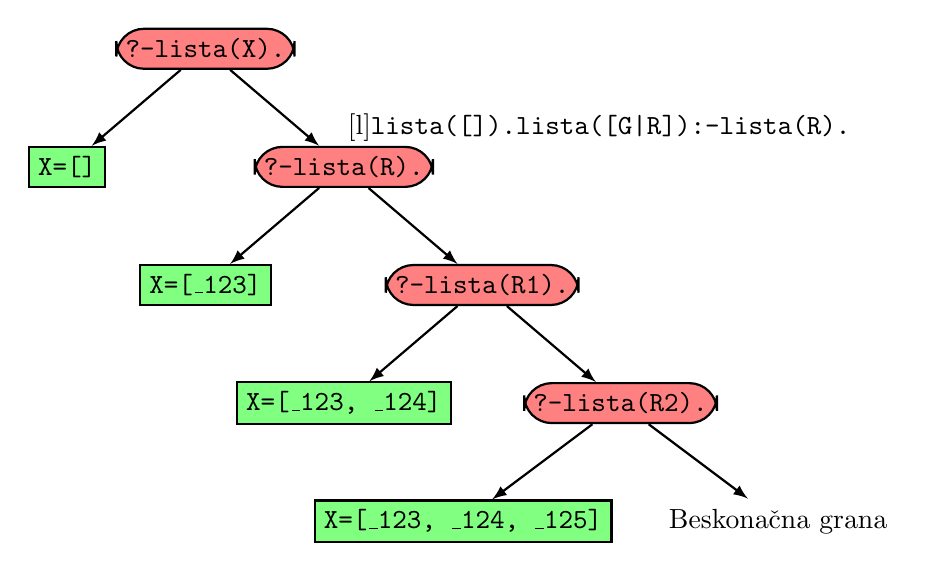
\begin{tikzpicture}[thick, -latex, smooth,%
	sibling distance=10em, 
	question/.style = {shape=rectangle, rounded corners=10pt, draw, align=left, fill=red!50},
	true/.style = {shape=rectangle, draw, align=left, fill=green!50},
	]
\tikzstyle{level 4}=[sibling distance=4cm]
\node[question] {\texttt{?-lista(X).}}
	child{ node[true] {\texttt{X=[]}}
	}
	child{ node[question] {\texttt{?-lista(R).}}
		child{ node[true] {\texttt{X=[\_123]}}
		}
		child{ node[question] {\texttt{?-lista(R1).}}
			child{ node[true] {\texttt{X=[\_123, \_124]}}
			}
			child{ node[question] {\texttt{?-lista(R2).}}
				child{ node[true] {\texttt{X=[\_123, \_124, \_125]}}
				}
				child{ node {Beskonačna grana}
				}
			}
		}
	};
\node at (5, -1) {\makecell[l]{\texttt{lista([]).} \\ \texttt{lista([G|R]):-lista(R).}}};
\end{tikzpicture}%
}
\end{example}
\end{boxprimer}
\columnbreak
{\bf Terminologija} \\
Stablo izvođenja -- stablo pretrage. Ono se sastoji iz grana i čvorova. Grana u stablu izvođenja može biti konačna ili beskonačna. Stablo izvođenja je konačno ako su sve grane u njemu konačne, u suprotnom je beskonačno.\\
{\it Čvorovi} koji su označeni upitom (ciljem) nazivaju se {\bf nezavršenim}. (Iz njih se izvode sledeći čvorovi). {\it Listovi} u stablu izvođenja nazivaju se {\bf završnim} čvorovima. {\it Grane} koje vode do završnih čvorova su {\bf konačne}. Grane koje nemaju završne čvorove su {\bf beskonačne}. \\
Ako završni čvor {\it daje rešenje}, naziva se {\bf čvor uspeha} (označen zelenom bojom), a odgovarajuća grana je {\bf grana uspeha}. Završni čvor koji ne predstavlja rešenje je {\bf čvor neuspeha} (označen crvenom bojom), a odgovarajuća grana je {\bf grana neuspeha}.
\end{multicols}

{\bf Veza stabla izvođenja i metoda rezolucije} \\
U smislu {\it deklarativne} semantike, stablo izvođenja odgovara poretku primene pravila rezolucije na postojeći skup činjenica i pravila. U smislu {\it proceduralne} semantike, stablo izvođenja odgovara procesu ispunjavanja ciljeva i podciljeva. Redosled činjenica i pravila u bazi znanja određuje redosled ispunjavanja ciljeva i izgled stabla izvodjenja. 
\\
S obzirom da su sve klauze Hornove, proces izvođenja je relativno jednostavan, ali efikasnost može i dalje da bude problem. Implementacija rezoluije može da se ostvari izvođenjem u širinu i izvođenjem u dubinu. Izvođenjem u širinu, radi se paralelno na svim podciljevima datog cilja, dok se izvođenjem u dubinu najpre izvede jedan podcilj, pa se dalje nastavlja sa ostalim podciljevima. Koja implementacija bi bila bolja?
\\
U Prologu je implementacija ostvarena izvođenjem u dubinu, jer su na taj način manji memorijski zahtevi. To znači da redosled tvrđenja u bazi znanja utiče i na efikasnost pronalaženja rešenja. Takođe, redosled može da utiče i na konačnost najlevlje grane, pa time i na to da li će rešenje uopšte biti pronađeno.
\\
{\bf Način obilaska stabla izvođenja i nalaženje rešenja}
Pomoću stabla izvođenja potpuno je određen prostor izvođenja za jedan cilj. Njega čine svi putevi koji vode od korena stabla do njegovih čvorova.

\begin{boxprimer}
\begin{example} \\
\resizebox{.8\textwidth}{!}{
\begin{tikzpicture}[thick, -latex,%
	sibling distance=3cm, 
	question/.style = {shape=rectangle, rounded corners=10pt, draw, align=left, fill=red!50},
	true/.style = {shape=rectangle, draw, align=left, fill=green!50},
	false/.style = {shape=rectangle, draw, align=left, fill=red!50}
	]
\tikzstyle{level 1}=[sibling distance=5cm]
\tikzstyle{level 2}=[sibling distance=5cm, level distance = 3cm]
\tikzstyle{level 3}=[sibling distance=3cm, level distance = 3cm]

\node[question] at (0,0)  {\texttt{?-hirurg(X)}}
	child{ node[question] {\texttt{?-lekar(X), operise(X)}}
		child{ node[question] {\makecell{\texttt{?-operise(X)},\\ \texttt{X=marko}}}
			child{ node[true] {\makecell{\texttt{X=marko},\\ \texttt{X=marko}}}
			}
			child{ node[false] {\makecell{\texttt{X=marko},\\ \texttt{X=milan}}}
			}
		}
		child{node[question] {\makecell{\texttt{?-operise(X)},\\ \texttt{X=stanko}}}
			child{ node[false] {\makecell{\texttt{X=stanko},\\ \texttt{X=marko}}}
			}
			child{ node[false] {\makecell{\texttt{X=stanko},\\ \texttt{X=milan}}}
			}
		}
		child{node[question] {\makecell{\texttt{?-operise(X)},\\ \texttt{X=milan}}}
			child{ node[false] {\makecell{\texttt{X=milan},\\ \texttt{X=marko}}}
			}
			child{ node[true] {\makecell{\texttt{X=milan},\\ \texttt{X=milan}}}
			}
		}
	}
	child{ node[true] {\texttt{X=petar}}
	};
%\draw[ thin,color=gray] (-10,-8) grid (5,0);
%\draw (0,0) node[circle, draw, color=red] {};
\draw [cyan] plot [smooth, tension=0.5] 
	coordinates {
		(-1.5,0.5) (-1,0) (-3, -1.5) (-6, -3.2) (-9, -4) (-10,-7) (-10, -8.5) (-8, -8.5) (-7.5, -5.5) %prvo spustanje
		(-7, -8.5) (-5,-8.5) %oko x marko x milan
		 (-6,-5.5) (-6,-4) (-3,-2) %vratili se u lekar, operise
		(-3, -3.5) (-4, -4) (-4, -5.3)
		(-5, -7) (-5,-8.5) (-3, -8.5) (-3,-7)%okruzili stanko marko
		(-2.5, -5.5) (-2, -7) %popeli se do operise stanko i spustili do stanko milan
		(-2, -8.5) (0, -8.5) (0, -7) % okruzili stanko milan i popeli se do operise stanko
		 (-1, -5.3) (-1, -4) 
		(-2, -3.5) (-2,-2)
		(1,-4) (1,-5.3)
		(0, -7) (0, -8.5) (2, -8.5) (2.5, -5.5) (3, -8.5) (5, -8.5) 
		 (4, -5.3) (4, -4) (1.5, -3.5) (-1,-2)
		(-1.5, -1.5) (0, -0.5)
		(1.5, -1.5) (2.5, -2) (3.5, -2) (3, -1) (1,-0.5) (2, 0.5)
	};
	%precrtano
\draw[gray!20, thin, - ]  (-5,-8.5) -- (-7,-6.5);
\draw[gray!20, thin, - ]  (-7,-8.5) -- (-5,-6.5);

\draw[gray!20, thin, - ]  (-5,-8.5) -- (-3,-6.5);
\draw[gray!20, thin, - ]  (-3,-8.5) -- (-5,-6.5);

\draw[gray!20, thin, - ]  (-2,-8.5) -- (0,-6.5);
\draw[gray!20, thin, - ]  (0,-8.5) -- (-2,-6.5);

\draw[gray!20, thin, - ]  (0,-8.5) -- (2,-6.5);
\draw[gray!20, thin, - ]  (2,-8.5) -- (0,-6.5);

\draw[red, very thick, -latex] (-8, -8) -- (-7.5,-5.5);
\draw[red, very thick, -latex] plot [smooth, tension=0.5] 
	coordinates {
	(-6, -7) (-6.5,-5.5) (-3,-2)
	};
\draw[red, very thick, -latex] (-3, -8) -- (-2.5,-5.5);
\draw[red, very thick, -latex] plot [smooth, tension=0.5] 
	coordinates {
	(-1, -7) (-1,-5.5) (-2,-2)
	};
\draw[red, very thick, -latex] (2, -8) -- (2.5,-5.5);
\draw[red, very thick, -latex] plot [smooth, tension=0.5] 
	coordinates {
	(4, -7) (4,-4) (-1,-2) (0, -0.5)
	};
\draw[red, very thick, -latex] (2, -1.1) -- (1,-0.3);

\end{tikzpicture}%
}
\end{example}
\end{boxprimer}

Kako je redosled izvođenja poznat i deterministički određen, to se može iskoristiti za dobijanje na efikasnosti Prolog programa time što se činjenice i pravila u bazi znanja ređaju u odgovarajućem redosledu. Takođe, na efikasnost utiče i davanje pogodnog redosleda podciljeva u pravilima. Ovo narušava pravila deklarativnosti po kojima redosled ne bi trebao da utiče na izvršavanje programa.

\subsection{Operator sečenja}
Sinonimi: operator sečenja, \texttt{cut} operator, rez operator, operator odsecanja.\\
To je sistemski operator koji omogućava brže izvršavanje programa i uštedu memorijskog prostora kroz eksplicitnu kontrolu backtracking-s. Ovaj operator je zapravo {\bf cilj koji uvek uspeva}. Operator sečenja odseca pojedine grane na stablu pretraživanja, pa samim tim smanjuje prostor pretraživanja. To omogućava brže nalaženje rešenja. U isto vreme ne moraju se pamtiti mnogoprojne tačke prilikom traženja sa vraćanjem, što dovodi do uštede memorijskog prostora.
\\
Neka imamo tvrđenje: \texttt{A :- B1, B2, \ldots, Bk, !, \ldots, Bm}\\
Kada se neki cilj G unifikuje sa A, aktivira se prethodno tvrđenje. Tada se cilj G naziva roditeljski cilj za A. Kada se dođe do reza, uspeli su podciljevi: B1, B2, \ldots, Bk. Sečenje uspeva i rešenje B1, B2, \ldots, Bk se ``zamrzava'', tj. predikat onemogućava traženje alternativnih rešenja. Takođe se onemogućava ujedinjavanje cilja G sa glavom nekog drugog predikata koji je u bazi podataka iza navedenog tvrđenja.
 
\begin{boxprimer}
\begin{example}
\begin{verbatim}
A :- P, Q, R, !, S, T.
A :- U.
G :- L, A, D.
?- G.
\end{verbatim}
U startu, traženje sa vraćanjem moguće je samo za P, Q, R. Kad uspe R uspeva i sečenje i alternativna rešenja se više ne traže. Alternativno rešenje: \texttt{A :- U}, takođe se ne razmatra. Alternativna rešenja su moguća između S i T, tj desno od operatora sečenja je moguć backtracking.
Ukoliko se ne nađe rešenje za fiksirane vrednosti P, Q, R, onda je dozvoljen backtracking.
\end{example}
\end{boxprimer}

\begin{boxprimer}
\begin{example} \\
\resizebox{.8\textwidth}{!}{
\begin{tikzpicture}[thick, -latex,%
	sibling distance=3cm, 
	question/.style = {shape=rectangle, rounded corners=10pt, draw, align=left, fill=red!50},
	true/.style = {shape=rectangle, draw, align=left, fill=green!50},
	false/.style = {shape=rectangle, draw, align=left, fill=red!50}
	]
\tikzstyle{level 1}=[sibling distance=3cm]
\tikzstyle{level 2}=[sibling distance=5cm]
\tikzstyle{level 3}=[sibling distance=7.5cm, level distance = 2.5cm]
\tikzstyle{level 4}=[sibling distance=2.5cm, level distance = 2.5cm]
\node [question]{\texttt{?-objekat(X).}}
	child{node[question] {\texttt{?-zivo\_bice(X).}}
		child{node[question]  (g) {\makecell[l]{\texttt{?-razmozava\_se(X)},\\ \texttt{raste(X)} }}
			child{node[question] { \texttt{?X=biljka, raste(X)}}
				child{node[true] {
					\makecell[l]{\texttt{X=biljka},\\ \texttt{X=biljka}}}}
				child{node[false] {
					\makecell[l]{\texttt{X=biljka},\\ \texttt{X=plima}}}}
				child{node[false] {
					\makecell[l]{\texttt{X=biljka},\\ \texttt{X=zivotinja}}}}
			}
			child{node[question] {\texttt{?X=zivotinja, raste(X)}}
				child{node[false] {
					\makecell[l]{\texttt{X=zivotinja},\\ \texttt{X=biljka}}}}
				child{node[false] {
					\makecell[l]{\texttt{X=zivotinja},\\ \texttt{X=plima}}}}
				child{node[true] {
					\makecell[l]{\texttt{X=zivotinja},\\ \texttt{X=zivotinja}}}}
			}
		}
		child{node[true] {\texttt{X=ptica}}
		}
	}
	child{node[true]  {\texttt{X=covek}}};
	
\draw[cyan, -, thin] plot [smooth, tension=0.5] coordinates{
	(-4,-9) (-2,-4) (0, -2.5) (3, -2)
};
\draw[cyan!70, -, thin] (-2,-4.5) -- (0,-3);
\draw[cyan!70, -, thin] (-2, -5) -- (1.5, -2.5);
\draw[cyan!70, -, thin] (-2.5, -6) -- (3, -2);
\draw[cyan!70, -, thin] (-3, -7) -- (3,-2.5);
\draw[cyan!70, -, thin] (-3.5, -8) -- (3, -3.5);
\draw[cyan!70, -, thin] (-3,-8) -- (3, -4);
\draw[cyan!70, -, thin] (-2,-8) -- (3, -5);
\draw[cyan!70, -, thin] (-1,-8) -- (3, -6);
\draw[cyan!70, -, thin] (0,-8) -- (3, -7);
%pomocni objekti
%\draw[ thin,color=gray] (-10,-8) grid (5,0);
%\draw (0,0) node[circle, draw, color=red] {};

\node [left = of g] {\makecell[l]{
\texttt{objekat(X):-zivo\_bice(X).}\\
\texttt{objekat(covek).}\\
\texttt{zivo\_bice(X):-razmnozava\_se(X),}\\
\tab \tab \tab \texttt{raste(X).}\\
\texttt{zivo\_bice(ptica).}\\
\texttt{raste(biljka).}\\
\texttt{raste(plima).}\\
\texttt{raste(zivotinja).}\\
\texttt{razmnozava\_se(biljka).}\\
\texttt{razmnozava\_se(zivotinja).}
}};
\end{tikzpicture}%
}
\end{example}
\end{boxprimer}

Predikat sečenja može se uporediti sa GOTO-naredbom u proceduralnim jezicima. Narušava deklarativni stil programiranja i može da proizvede neželjene efekte (greške). Pogrešna upotreba operatora sečenja je najčešći uzrok grešaka programiranja u Prologu. Ipak, ovaj predikat je često neophodan za dobijanje efikasnih rešenja i treba ga koristiti (ali oprezno!). Ako se predikat sečenja upotrebljava tako da ne narušava deklarativno svojstvo predikata tj. ne menja njegovu semantiku niti skup rešenja (već samo pojačava njegova deterministička svojstva i ubrzava proces izračunavanja), onda se naziva {\bf zeleni predikat sečenja}. Treba biti veoma oprezan sa upotrebom predikata sečenja.

\begin{boxprimer}
\begin{example}
Primena operatora sečenja\\
Kada želimo da saopštimo Prologu: ``Nađeno je potrebno rešenje, ne treba dalje tražiti!''
\begin{Verbatim}
auto(mercedes, 200000, 10000).
auto(skoda, 100000, 5000).
auto(fiat, 50000, 4000).
auto(bmv, 12000, 12000).
zadovoljava(M) :- auto(M, K, C), C<5000, !.
\end{Verbatim}
\end{example}
\end{boxprimer} 

\begin{boxprimer}
\begin{example}
Primena operatora sečenja\\
Kada želimo da saopštimo Prologu:``Nađeno je jedinstveno rešenje i ne treba dalje tražiti!''
\begin{Verbatim}
kolicnik(N1, N2, Rez):-ceo_broj(Rez),
		P1 is Rez*N2,
		P2 is (Rez+1)*N2,
		P1=<N1, P2>N1, !.
ceo_broj(0).
ceo_broj(X) :- ceo_broj(Y), X is Y+1.
\end{Verbatim}
\end{example}
\end{boxprimer} 

\begin{boxprimer}
\begin{example}
Primena operatora sečenja\\
Kada želimo da saopštimo Prologu:``Na pogrešnom si putu, završiti pokušaj zadovoljenja cilja!''.
\begin{Verbatim}
inostrani(dzon).
inostrani(matrin).
dohodak(dzon, 5000).
dohodak(matrin, 10000).
dohodak(pera, 20000).
placa_porez(X) :- inostrani(X), !, fail.
placa_porez(X) :- dohodak(X,D), D>10000.
\end{Verbatim}
\end{example}
\end{boxprimer} 
Koristi se u kombinaciji sa \texttt{fail}-predikatom. Može samo da se koristi za proverne svrhe, ne i za generisanje rešenja.

\subsection{Svojstva Prologa}
Prolog nije čist deklarativni jezik (kontrola rezolucije i backtracking-a). On je restrikcija logike prvog reda na formule koje se mogu svesti na Hornove klauze. Hornovim klauzama ne mogu se opisati sva tvrđenja logike prvog reda. 
\\
Prolog može da dokaže da je neki cilj ispunjen, ali ne i da neki cilj nije ispunjen. To je posledica oblika Hornovih klauza $A:-B_1, B_2, \ldots, B_n$ ako su sve $B_i$ tačne, možemo da zaključimo da je $A$ tačno, ali ne postoji način da zaključimo da $A$ nije tačno. Prema tome, ukoliko Prolog ne može da dokaže da je neki cilj ispunjen, on prijavljuje da cilj nije ispunjen, iako je to zapravo nemogućnost dokazivanja tačnosti, a ne dokazivanje netačnosti. Preciznije, Prolog je {\bf true/fail }sistem, a ne true/false i to treba imati na umu.
\\
{\bf Operator NOT} nije operator negacije u smislu logičke negacije. Naziva se {\bf ``negacija kao neuspeh''}, \texttt{not(cilj)} uspeva ukoliko \texttt{cilj} ne uspeva. Zapravo, logičko NOT ne može da bude sastavni deo Prologa što je posledica oblika Hornovih klauza. To znači da, ukoliko imamo na primer naredni oblik \texttt{not(not(cilj))} to ne mora da bude ekvivalentno sa \texttt{cilj}, što može da dovede do raznih problema i neočekivanih rezultata. Zbog toga i sa upotrebom operatora NOT treba biti veoma pažljiv i koristiti ga samo za instancirane promenljive.

\begin{boxprimer}
\begin{example} {\bf operator not}

\begin{multicols}{2}

\begin{Verbatim}
vozac(janko).
vozac(marko).
vozac(petar).
pije(janko).
pije(marko).
dobar_vozac(X) :- not(pije(X)), vozac(X).
\end{Verbatim}
\columnbreak
\begin{Verbatim}
?-dobar_vozac(X).
no
?-dobar_vozac(petar).
yes
?-pije(X).
X=janko;
X=marko;
no
?-not(not(pije(X))).
yes
\end{Verbatim}

\end{multicols}

\end{example}
\end{boxprimer}

\begin{boxprimer}
\begin{example} {\bf operator NOT}

\begin{multicols}{2}

\begin{Verbatim}
vozac(janko).
vozac(marko).
vozac(petar).
pije(janko).
pije(marko).
dobar_vozac(X) :- vozac(X),not(pije(X)).
\end{Verbatim}
\columnbreak

\begin{Verbatim}
?-dobar_vozac(X).
X=petar;
no
?-dobar_vozac(petar).
yes
\end{Verbatim}

\end{multicols}

\end{example}
\end{boxprimer}

\begin{boxprimer}
\begin{multicols}{2}
Objasniti naredne rezultate:
\begin{Verbatim}
?- not(X==1), X=1.
X = 1
yes
?- X=1, not(X==1).
no
\end{Verbatim}

\columnbreak
X nije instancirano, pa stoga nije identično jedinici, i not operator uspeva.
Da bi uspeo i drugi cilj, X se unifikuje sa 1.
\begin{Verbatim}
?- not(X==1), X=1.
X = 1
yes
\end{Verbatim}
U ovom slučaju, X se najpre unifikuje sa 1, i kako je $1 == 1$ not ne uspeva.
\begin{Verbatim}
?- X=1, not(X==1).
no
\end{Verbatim}
\end{multicols}
\end{boxprimer}

{\bf Generisanje efikasnih algoritama}\\
Osnovni cilj logičkog programiranja je da se obezbedi programiranje takvo da programer da specifikaciju šta program treba da uradi bez specifikacije na koji način to treba da se ostvari. Visok nivo apstrakcije i deklarativnosti nosi sa sobom cenu neefikasnosti. 
\\
Sortiranje može jednostavno da se definiše kao generisanje permutacije i provera da li je permutacija sortirana. Na primer, kriterijum da li je niz sortiran može u Prologu da se napise:
\begin{Verbatim}
sorted([]).
sorted([X]).
sorted([X, Y | List]) :- X =< Y, sorted([Y|List]).
\end{Verbatim}
Međutim, sam algoritam sortiranja je potpuno neefikasan: problem je što nije dat način na koji da se izvrši sortiranje i jedini način da se to ostvari je enumeracijom svih permutacija liste dok se ne kreira ona permutacija koja zadovoljava svojstvo sortiranosti liste. Zapravo, ne postoji način da se opis sortiranosti liste prevede u efikasan način sortiranja elemenata liste -- rezolucija ne može da generiše efikasan algoritam. Prema tome, ako želimo efikasno izvršavanje, moramo da damo specifikaciju algoritma i u Prologu. Možda ćemo jednog dana doći do tačke da su sami programski sistemi u mogućnosti da otkriju dobre algoritme iz deklarativnih specifikacija, ali to još uvek nije slučaj.
\\
{\bf Moduli}\\
Kreiranje mogula u Prologu propisano je ISO standardom, ali ne podržavaju svi kompajleri ovo svojstvo što značajno otežava razvoj kompleksnog softvera. Postoje nekompatibilnosti između sistema modula različitih Prolog kompajlera. Takođe, većina kompajlera implementira i dodatne funkcionalnosti koje nisu podržane standardom, što onemogućava kompatibilnost između kompajlera.
\begin{itemize}
\item Prolog je Tjuring-kompletan jezik, to se može pokazati korišćenjem Prologa da simulira Tjuringovu mašinu.
\item Prolog je netipiziran jezik, postoje razni pokušaji uvođenja tipova u Prolog.
\item Prolog ima mehanizam prepoznavanja i optimizacije repne rekurzije, tako da se ona izvršava jednako efikasno kao i petlje u proceduralnim jezicima.
\item Predikati višeg reda su predikati koji uzimaju jedan ili više predikata kao svoje argumente. To izlazi iz okvira logike prvog reda, ali ISO standard propisuje neke predikate višeg reda (na primer predikat \texttt{call})
\end{itemize}

\subsection{Programiranje ograničenja u logičkom programiranju}

Programiranje ograničenja je deklarativno programiranje. U njemu se relacije između promenljivih zadaju u vidu ograničenja. Od sistema se zatim očekuje da izračuna rešenje, tj da izračuna vrednosti promenljivih koje zadovoljavaju data ograničenja. Ograničenja se razlikuju od ograničenja u imperativnoj paradigmi. Na primer, $x<y$ u imperativnoj paradigmi se evaluira u tačno ili netačno, dok u paradigmi ograničenja zadaje relaciju između objekata $x$ i $y$ koja mora da važi. 
\\
Ograničenja mogu da budu različitih vrsta, na primer, ograničenja iskazne logike (A ili B je tačno), linearna ograničenja ($x<15$), ograničenja nad konačnim domenima. Rešavanje ograničenja vrši se različitim rešavačima, npr SAT i SMT. Programiranje ograničenja ima primene pre svega u operacionim istraživanjima (tj u rešavanju kombinatornih i optimizacionih problema). 

\subsubsection{B-Prolog}

\href{http://www.picat-lang.org/bprolog/}{B-Prolog (http://www.picat-lang.org/bprolog/)}\\
Nastao je 1994. Komercijalni je proizvod, ali se može koristiti za učenje i istraživanja besplatno. Implementira ISO standard Prologa, ali i razna proširenja. B-Prolog ima bogat sistem za programiranje ograničenja. Podržava programiranje ograničenja na različitim domenima, npr na konačnom i iskaznom domenu.

Programiranje ograničenja se sastoji od tri dela:
\begin{itemize}
\item Generisanje promenljivih i njihovih domena.
\item Generisanje ograničenja nad promenljivama
\item Obeležavanje (labeling) -- instanciranje promenljivih
\end{itemize}

Za programiranje ograničenja uvode se novi predikati, koje ćemo razmotriti kroz primere.
\\
Generisanje promenljivih i njihovih domena:
\begin{itemize}
\item Definisanje domena: \texttt{Vars in D} ili \texttt{Vars :: D}
\item \texttt{D} se definiše kao \texttt{pocetak..korak..kraj}
\item \texttt{1..5..20} definiše domen \texttt{1, 6, 11, 16}
\item Korak nije obavezan, podrazumeva se da je jedan.
\item Postoje predikati za opšta ograničenja, a mogu se zadavati numerička ograničenja.
\item Numerička počinju sa \texttt{\#}, npr \texttt{\#<}, \texttt{\#<=},\ldots
\item Labeling se odnosi na instanciranje promenljivih i na njihovo prikazivanje.
\end{itemize}

\begin{boxprimer}
\begin{multicols}{2}
\begin{Verbatim}
?- X in 1..10, Y in 5..2..30, X#>=Y, labeling(X).
X = 5
Y = 5 ?;
X = 6
Y = 5 ?;
X = 7
Y = _0490::[5,7] ?;
X = 8
Y = _0490::[5,7] ?;
X = 9
Y = _0490::[5,7,9] ?;
X = 10
Y = _0490::[5,7,9] ?;
no
\end{Verbatim}
\columnbreak
\makecell[l]{
\\
\\
Promenljive: X i Y \\
Domeni: X je bilo koji broj od 1 do 10\\
\tab Y su neparni brojevi od 5 do 30 \\
Ograničenje: $X\ge Y$\\
Instanciranje: po X
}
\end{multicols}
\end{boxprimer}

\begin{boxprimer}
\begin{multicols}{2}

\begin{Verbatim}
?- X in 1..10, Y in 5..2..30, X#>=Y, labeling(X), labeling(Y).
X = 5
Y = 5 ?;
X = 6
Y = 5 ?;
X = 7
Y = 7 ?;
X = 8
Y = 5 ?;
...
\end{Verbatim}
\columnbreak
\makecell[l]{
\\
\\
Promenljive: X i Y \\
Domeni: X je bilo koji broj od 1 do 10\\
\tab Y su neparni brojevi od 5 do 30 \\
Ograničenje: $X\ge Y$\\
Instanciranje: po X i Y
}
\end{multicols}
\end{boxprimer}


\begin{boxprimer}
\begin{Verbatim}
sendmoremoney(Vars) :- Vars = [S,E,N,D,M,O,R,Y], %generisanje promenljivih
	Vars :: 0..9,                            %definisanje domena
	S #\= 0,                                 %ogranicenja
	M#\=0,
	all_different(Vars),
	             1000*S + 100*E + 10*N + D
	+            1000*M + 100*O + 10*N + E
	#= 10000*M + 1000*O + 100*N + 10*E + Y,
	labeling(Vars).                          %instanciranje

| ?- consult(primer1).
| ?- sendmoremoney(Vars).
Vars = [9,5,6,7,1,0,8,2] ?;
no
\end{Verbatim}
\end{boxprimer}

\begin{boxprimer}
\begin{multicols}{2}
\begin{Verbatim}
|X1 X2 | |
|X3 X4 X5|
| | X6 X7|
crossword(Vars):-
	Vars=[X1,X2,X3,X4,X5,X6,X7],
	Words2=[(0’I,0’N),
		(0’I,0’F),	%IF
		(0’A,0’S),	%AS
		(0’G,0’O),	%GO
		(0’T,0’O)],       %TO
	Words3=[(0’F,0’U,0’N),    %FUN
		(0’T,0’A,0’D),    %TAD
		(0’N,0’A,0’G),    %NAG
		(0’S,0’A,0’G)],   %SAG
	[(X1,X2),(X1,X3),(X5,X7),(X6,X7)] in Words2,
	[(X3,X4,X5),(X2,X4,X6)] in Words3,
	labeling(Vars),
	format("~s~n",[Vars]).
\end{Verbatim}
\columnbreak
\begin{Verbatim}
| ?- consult(primer2).
| ?- crossword(Vars).
ASSAGGO
Vars = [65,83,83,65,71,71,79] ?;
INNAGGO
Vars = [73,78,78,65,71,71,79] ?;
no
\end{Verbatim}
\end{multicols}
\end{boxprimer}

\begin{boxprimer}
\begin{multicols}{2}
\begin{Verbatim}
queens(N):-
	length(Qs,N),
	Qs :: 1..N,
	foreach(I in 1..N-1, J in I+1..N,
		(Qs[I] #\= Qs[J],
		abs(Qs[I]-Qs[J]) #\= J-I)),
	labeling([ff],Qs),
	writeln(Qs).
\end{Verbatim}
\columnbreak
\begin{Verbatim}
| ?- consult(primer3).
| ?- queens(5).
[1,3,5,2,4]
yes
| ?- queens(8).
[1,5,8,6,3,7,2,4]
yes
| ?- queens(10).
[1,3,6,9,7,10,4,2,5,8]
yes
| ?- queens(15).
[1,3,5,14,11,4,10,7,13,15,2,8,6,9,12]
yes
\end{Verbatim}
\end{multicols}
\end{boxprimer}


\end{document}
